
%% bare_conf.tex
%% V1.3
%% 2007/01/11
%% by Michael Shell
%% See:
%% http://www.michaelshell.org/
%% for current contact information.
%%
%% This is a skeleton file demonstrating the use of IEEEtran.cls
%% (requires IEEEtran.cls version 1.7 or later) with an IEEE conference paper.
%%
%% Support sites:
%% http://www.michaelshell.org/tex/ieeetran/
%% http://www.ctan.org/tex-archive/macros/latex/contrib/IEEEtran/
%% and
%% http://www.ieee.org/

%%*************************************************************************
%% Legal Notice:
%% This code is offered as-is without any warranty either expressed or
%% implied; without even the implied warranty of MERCHANTABILITY or
%% FITNESS FOR A PARTICULAR PURPOSE! 
%% User assumes all risk.
%% In no event shall IEEE or any contributor to this code be liable for
%% any damages or losses, including, but not limited to, incidental,
%% consequential, or any other damages, resulting from the use or misuse
%% of any information contained here.
%%
%% All comments are the opinions of their respective authors and are not
%% necessarily endorsed by the IEEE.
%%
%% This work is distributed under the LaTeX Project Public License (LPPL)
%% ( http://www.latex-project.org/ ) version 1.3, and may be freely used,
%% distributed and modified. A copy of the LPPL, version 1.3, is included
%% in the base LaTeX documentation of all distributions of LaTeX released
%% 2003/12/01 or later.
%% Retain all contribution notices and credits.
%% ** Modified files should be clearly indicated as such, including  **
%% ** renaming them and changing author support contact information. **
%%
%% File list of work: IEEEtran.cls, IEEEtran_HOWTO.pdf, bare_adv.tex,
%%                    bare_conf.tex, bare_jrnl.tex, bare_jrnl_compsoc.tex
%%*************************************************************************

% *** Authors should verify (and, if needed, correct) their LaTeX system  ***
% *** with the testflow diagnostic prior to trusting their LaTeX platform ***
% *** with production work. IEEE's font choices can trigger bugs that do  ***
% *** not appear when using other class files.                            ***
% The testflow support page is at:
% http://www.michaelshell.org/tex/testflow/



% Note that the a4paper option is mainly intended so that authors in
% countries using A4 can easily print to A4 and see how their papers will
% look in print - the typesetting of the document will not typically be
% affected with changes in paper size (but the bottom and side margins will).
% Use the testflow package mentioned above to verify correct handling of
% both paper sizes by the user's LaTeX system.
%
% Also note that the "draftcls" or "draftclsnofoot", not "draft", option
% should be used if it is desired that the figures are to be displayed in
% draft mode.
%
\documentclass[conference]{IEEEtran}
% Add the compsoc option for Computer Society conferences.
%
% If IEEEtran.cls has not been installed into the LaTeX system files,
% manually specify the path to it like:
% \documentclass[conference]{../sty/IEEEtran}





% Some very useful LaTeX packages include:
% (uncomment the ones you want to load)


% *** MISC UTILITY PACKAGES ***
%
%\usepackage{ifpdf}
% Heiko Oberdiek's ifpdf.sty is very useful if you need conditional
% compilation based on whether the output is pdf or dvi.
% usage:
% \ifpdf
%   % pdf code
% \else
%   % dvi code
% \fi
% The latest version of ifpdf.sty can be obtained from:
% http://www.ctan.org/tex-archive/macros/latex/contrib/oberdiek/
% Also, note that IEEEtran.cls V1.7 and later provides a builtin
% \ifCLASSINFOpdf conditional that works the same way.
% When switching from latex to pdflatex and vice-versa, the compiler may
% have to be run twice to clear warning/error messages.






% *** CITATION PACKAGES ***
%
\usepackage{cite}
% cite.sty was written by Donald Arseneau
% V1.6 and later of IEEEtran pre-defines the format of the cite.sty package
% \cite{} output to follow that of IEEE. Loading the cite package will
% result in citation numbers being automatically sorted and properly
% "compressed/ranged". e.g., [1], [9], [2], [7], [5], [6] without using
% cite.sty will become [1], [2], [5]--[7], [9] using cite.sty. cite.sty's
% \cite will automatically add leading space, if needed. Use cite.sty's
% noadjust option (cite.sty V3.8 and later) if you want to turn this off.
% cite.sty is already installed on most LaTeX systems. Be sure and use
% version 4.0 (2003-05-27) and later if using hyperref.sty. cite.sty does
% not currently provide for hyperlinked citations.
% The latest version can be obtained at:
% http://www.ctan.org/tex-archive/macros/latex/contrib/cite/
% The documentation is contained in the cite.sty file itself.






% *** GRAPHICS RELATED PACKAGES ***
%
\ifCLASSINFOpdf
  % \usepackage[pdftex]{graphicx}
  % declare the path(s) where your graphic files are
  % \graphicspath{{../pdf/}{../jpeg/}}
  % and their extensions so you won't have to specify these with
  % every instance of \includegraphics
  % \DeclareGraphicsExtensions{.pdf,.jpeg,.png}
\else
  % or other class option (dvipsone, dvipdf, if not using dvips). graphicx
  % will default to the driver specified in the system graphics.cfg if no
  % driver is specified.
  % \usepackage[dvips]{graphicx}
  % declare the path(s) where your graphic files are
  % \graphicspath{{../eps/}}
  % and their extensions so you won't have to specify these with
  % every instance of \includegraphics
  % \DeclareGraphicsExtensions{.eps}
\fi
% graphicx was written by David Carlisle and Sebastian Rahtz. It is
% required if you want graphics, photos, etc. graphicx.sty is already
% installed on most LaTeX systems. The latest version and documentation can
% be obtained at: 
% http://www.ctan.org/tex-archive/macros/latex/required/graphics/
% Another good source of documentation is "Using Imported Graphics in
% LaTeX2e" by Keith Reckdahl which can be found as epslatex.ps or
% epslatex.pdf at: http://www.ctan.org/tex-archive/info/
%
% latex, and pdflatex in dvi mode, support graphics in encapsulated
% postscript (.eps) format. pdflatex in pdf mode supports graphics
% in .pdf, .jpeg, .png and .mps (metapost) formats. Users should ensure
% that all non-photo figures use a vector format (.eps, .pdf, .mps) and
% not a bitmapped formats (.jpeg, .png). IEEE frowns on bitmapped formats
% which can result in "jaggedy"/blurry rendering of lines and letters as
% well as large increases in file sizes.
%
% You can find documentation about the pdfTeX application at:
% http://www.tug.org/applications/pdftex





% *** MATH PACKAGES ***
%
%\usepackage[cmex10]{amsmath}
% A popular package from the American Mathematical Society that provides
% many useful and powerful commands for dealing with mathematics. If using
% it, be sure to load this package with the cmex10 option to ensure that
% only type 1 fonts will utilized at all point sizes. Without this option,
% it is possible that some math symbols, particularly those within
% footnotes, will be rendered in bitmap form which will result in a
% document that can not be IEEE Xplore compliant!
%
% Also, note that the amsmath package sets \interdisplaylinepenalty to 10000
% thus preventing page breaks from occurring within multiline equations. Use:
%\interdisplaylinepenalty=2500
% after loading amsmath to restore such page breaks as IEEEtran.cls normally
% does. amsmath.sty is already installed on most LaTeX systems. The latest
% version and documentation can be obtained at:
% http://www.ctan.org/tex-archive/macros/latex/required/amslatex/math/





% *** SPECIALIZED LIST PACKAGES ***
%
%\usepackage{algorithmic}
% algorithmic.sty was written by Peter Williams and Rogerio Brito.
% This package provides an algorithmic environment fo describing algorithms.
% You can use the algorithmic environment in-text or within a figure
% environment to provide for a floating algorithm. Do NOT use the algorithm
% floating environment provided by algorithm.sty (by the same authors) or
% algorithm2e.sty (by Christophe Fiorio) as IEEE does not use dedicated
% algorithm float types and packages that provide these will not provide
% correct IEEE style captions. The latest version and documentation of
% algorithmic.sty can be obtained at:
% http://www.ctan.org/tex-archive/macros/latex/contrib/algorithms/
% There is also a support site at:
% http://algorithms.berlios.de/index.html
% Also of interest may be the (relatively newer and more customizable)
% algorithmicx.sty package by Szasz Janos:
% http://www.ctan.org/tex-archive/macros/latex/contrib/algorithmicx/




% *** ALIGNMENT PACKAGES ***
%
%\usepackage{array}
% Frank Mittelbach's and David Carlisle's array.sty patches and improves
% the standard LaTeX2e array and tabular environments to provide better
% appearance and additional user controls. As the default LaTeX2e table
% generation code is lacking to the point of almost being broken with
% respect to the quality of the end results, all users are strongly
% advised to use an enhanced (at the very least that provided by array.sty)
% set of table tools. array.sty is already installed on most systems. The
% latest version and documentation can be obtained at:
% http://www.ctan.org/tex-archive/macros/latex/required/tools/


%\usepackage{mdwmath}
%\usepackage{mdwtab}
% Also highly recommended is Mark Wooding's extremely powerful MDW tools,
% especially mdwmath.sty and mdwtab.sty which are used to format equations
% and tables, respectively. The MDWtools set is already installed on most
% LaTeX systems. The lastest version and documentation is available at:
% http://www.ctan.org/tex-archive/macros/latex/contrib/mdwtools/


% IEEEtran contains the IEEEeqnarray family of commands that can be used to
% generate multiline equations as well as matrices, tables, etc., of high
% quality.


%\usepackage{eqparbox}
% Also of notable interest is Scott Pakin's eqparbox package for creating
% (automatically sized) equal width boxes - aka "natural width parboxes".
% Available at:
% http://www.ctan.org/tex-archive/macros/latex/contrib/eqparbox/





% *** SUBFIGURE PACKAGES ***
%\usepackage[tight,footnotesize]{subfigure}
% subfigure.sty was written by Steven Douglas Cochran. This package makes it
% easy to put subfigures in your figures. e.g., "Figure 1a and 1b". For IEEE
% work, it is a good idea to load it with the tight package option to reduce
% the amount of white space around the subfigures. subfigure.sty is already
% installed on most LaTeX systems. The latest version and documentation can
% be obtained at:
% http://www.ctan.org/tex-archive/obsolete/macros/latex/contrib/subfigure/
% subfigure.sty has been superceeded by subfig.sty.



%\usepackage[caption=false]{caption}
%\usepackage[font=footnotesize]{subfig}
% subfig.sty, also written by Steven Douglas Cochran, is the modern
% replacement for subfigure.sty. However, subfig.sty requires and
% automatically loads Axel Sommerfeldt's caption.sty which will override
% IEEEtran.cls handling of captions and this will result in nonIEEE style
% figure/table captions. To prevent this problem, be sure and preload
% caption.sty with its "caption=false" package option. This is will preserve
% IEEEtran.cls handing of captions. Version 1.3 (2005/06/28) and later 
% (recommended due to many improvements over 1.2) of subfig.sty supports
% the caption=false option directly:
%\usepackage[caption=false,font=footnotesize]{subfig}
%
% The latest version and documentation can be obtained at:
% http://www.ctan.org/tex-archive/macros/latex/contrib/subfig/
% The latest version and documentation of caption.sty can be obtained at:
% http://www.ctan.org/tex-archive/macros/latex/contrib/caption/




% *** FLOAT PACKAGES ***
%
%\usepackage{fixltx2e}
% fixltx2e, the successor to the earlier fix2col.sty, was written by
% Frank Mittelbach and David Carlisle. This package corrects a few problems
% in the LaTeX2e kernel, the most notable of which is that in current
% LaTeX2e releases, the ordering of single and double column floats is not
% guaranteed to be preserved. Thus, an unpatched LaTeX2e can allow a
% single column figure to be placed prior to an earlier double column
% figure. The latest version and documentation can be found at:
% http://www.ctan.org/tex-archive/macros/latex/base/



%\usepackage{stfloats}
% stfloats.sty was written by Sigitas Tolusis. This package gives LaTeX2e
% the ability to do double column floats at the bottom of the page as well
% as the top. (e.g., "\begin{figure*}[!b]" is not normally possible in
% LaTeX2e). It also provides a command:
%\fnbelowfloat
% to enable the placement of footnotes below bottom floats (the standard
% LaTeX2e kernel puts them above bottom floats). This is an invasive package
% which rewrites many portions of the LaTeX2e float routines. It may not work
% with other packages that modify the LaTeX2e float routines. The latest
% version and documentation can be obtained at:
% http://www.ctan.org/tex-archive/macros/latex/contrib/sttools/
% Documentation is contained in the stfloats.sty comments as well as in the
% presfull.pdf file. Do not use the stfloats baselinefloat ability as IEEE
% does not allow \baselineskip to stretch. Authors submitting work to the
% IEEE should note that IEEE rarely uses double column equations and
% that authors should try to avoid such use. Do not be tempted to use the
% cuted.sty or midfloat.sty packages (also by Sigitas Tolusis) as IEEE does
% not format its papers in such ways.





% *** PDF, URL AND HYPERLINK PACKAGES ***
%
%\usepackage{url}
% url.sty was written by Donald Arseneau. It provides better support for
% handling and breaking URLs. url.sty is already installed on most LaTeX
% systems. The latest version can be obtained at:
% http://www.ctan.org/tex-archive/macros/latex/contrib/misc/
% Read the url.sty source comments for usage information. Basically,
% \url{my_url_here}.





% *** Do not adjust lengths that control margins, column widths, etc. ***
% *** Do not use packages that alter fonts (such as pslatex).         ***
% There should be no need to do such things with IEEEtran.cls V1.6 and later.
% (Unless specifically asked to do so by the journal or conference you plan
% to submit to, of course. )


% correct bad hyphenation here
\hyphenation{op-tical net-works semi-conduc-tor}



\usepackage{graphicx}
\usepackage{listings}

\begin{document}

%
% paper title
% can use linebreaks \\ within to get better formatting as desired
\title{jFuzzyLogic: A Robust and Flexible Fuzzy-Logic Inference System Language Implementation}

% author names and affiliations
% use a multiple column layout for up to three different
% affiliations
\author{\IEEEauthorblockN{Pablo Cingolani}
\IEEEauthorblockA{School of Computer Science \\
McGill University \\
Montreal, Quebec, H3A-1A4, Canada \\
Email: pablo.cingolani@mcgill.ca}
\and
\IEEEauthorblockN{Jes\'us Alcal\'a-Fdez, {\it Member, IEEE}}
\IEEEauthorblockA{Department of Computer Science and Artificial Intelligence\\ 
University of Granada, CITIC-UGR\\
Granada, 18071, Spain\\
Email: jalcala@decsai.ugr.es}}

% conference papers do not typically use \thanks and this command
% is locked out in conference mode. If really needed, such as for
% the acknowledgment of grants, issue a \IEEEoverridecommandlockouts
% after \documentclass

% for over three affiliations, or if they all won't fit within the width
% of the page, use this alternative format:
% 
%\author{\IEEEauthorblockN{Michael Shell\IEEEauthorrefmark{1},
%Homer Simpson\IEEEauthorrefmark{2},
%James Kirk\IEEEauthorrefmark{3}, 
%Montgomery Scott\IEEEauthorrefmark{3} and
%Eldon Tyrell\IEEEauthorrefmark{4}}
%\IEEEauthorblockA{\IEEEauthorrefmark{1}School of Electrical and Computer Engineering\\
%Georgia Institute of Technology,
%Atlanta, Georgia 30332--0250\\ Email: see http://www.michaelshell.org/contact.html}
%\IEEEauthorblockA{\IEEEauthorrefmark{2}Twentieth Century Fox, Springfield, USA\\
%Email: homer@thesimpsons.com}
%\IEEEauthorblockA{\IEEEauthorrefmark{3}Starfleet Academy, San Francisco, California 96678-2391\\
%Telephone: (800) 555--1212, Fax: (888) 555--1212}
%\IEEEauthorblockA{\IEEEauthorrefmark{4}Tyrell Inc., 123 Replicant Street, Los Angeles, California 90210--4321}}

% use for special paper notices
%\IEEEspecialpapernotice{(Invited Paper)}

% make the title area
\maketitle

\begin{abstract}
%\boldmath
This work introduces jFuzzyLogic, an open source library for fuzzy systems which allow us to design Fuzzy Logic Controllers supporting the standard for Fuzzy Control Programming published by the International Electrotechnical Commission. 
This library is written in Java and is available as open source from jfuzzylogic.sourceforge.net. 
The use of jFuzzyLogic is illustrated through the analysis of one case study. 
\end{abstract}

% IEEEtran.cls defaults to using nonbold math in the Abstract.
% This preserves the distinction between vectors and scalars. However,
% if the conference you are submitting to favors bold math in the abstract,
% then you can use LaTeX's standard command \boldmath at the very start
% of the abstract to achieve this. Many IEEE journals/conferences frown on
% math in the abstract anyway.

% no keywords

% For peer review papers, you can put extra information on the cover
% page as needed:
% \ifCLASSOPTIONpeerreview
% \begin{center} \bfseries EDICS Category: 3-BBND \end{center}
% \fi
%
% For peerreview papers, this IEEEtran command inserts a page break and
% creates the second title. It will be ignored for other modes.
\IEEEpeerreviewmaketitle

\section{Introduction}
% no \IEEEPARstart

Fuzzy rule based systems (FRBSs) are one of the most important areas for the application of the Fuzzy Set Theory\cite{Zadeh65}. 
%Usually it is considered a model structure in the form of 
Classical rule based systems deal with IF-THEN rules.
FRBSs constitute an extension to classical systems, having antecedents and consequents composed of fuzzy logic statements.

A Fuzzy Logic Controller (FLC)~\cite{Lee90,DHR93,YF94,Bon94} is a FRBS composed of: 
	i-) a Knowledge Base that comprises the information used by the expert operator in the form of linguistic control rules; 
	ii-) a Fuzzification Interface, that transforms the crisp values of the input variables into fuzzy sets;
	iii-) an Inference System, that uses the fuzzy values from the Fuzzification Interface and the information from the Knowledge Base to perform the reasoning process and 
	iv-) the Defuzzification Interface, which takes the fuzzy action from the Inference System and translates it into crisp values for the control variables.

FLCs are suitable for engineering applications in which classical control strategies do not achieve good results or when it is too difficult to obtain a mathematical model.
FLCs usually have two characteristics: the need for human operator experience, and a strong non linearity.
Many real-world applications use FLCs~\cite{PDH97} such as mobile robot navigation \cite{MAA10,JCh2011}, air conditioning controllers \cite{Alc12,Cho11}, domotic control\cite{Cha12,AL05}, and industrial applications\cite{ZG2012,Demir12}.

FLCs are powerful for solving a wide range of problems, but their implementation requires a certain programming expertise.
In the last few years, many fuzzy logic software tools have been developed to reduce this task. 
Some are commercially distributed, for example MATLAB Fuzzy logic toolbox(www.mathworks.com), while a few are available as open source software (see section \ref{sec:stu}).

In this work, we introduce an open source Java library named jFuzzyLogic. 
This fuzzy systems library allows FLCs design and implementation, following the standard for Fuzzy Control Language (FCL) published by the International Electrotechnical Commission (IEC 61131-7)\cite{IEC}. 
The IEC-61131 norm is well known for defining the Programmable Controller Languages (PLC), commonly used in industrial applications.
In the part 7, this standard offers a well defined common understanding of the basic means to integrate fuzzy control applications in control systems.
It also defines a common language to exchange portable fuzzy control programs among different platforms.

The main goal of jFuzzyLogic is to bring the benefits of open source software and standardization to the fuzzy systems community. Our library offers several advantages:

\begin{itemize}

	\item Standardization, which reduces programming work and learning curve. This library contains the basic programming elements for the Standard IEC 61131-7, alleviating developers from boiler plate programming tasks.

	\item Extensibility, the object model and API allows to create a wide range of applications. This is of special interest for the research community.

	\item Platform independence, allows to develop and run on any hardware and operating system configuration that supports Java.

\end{itemize}

This work is arranged as follows.
The next section presents a comparison on non-commercial fuzzy software and the main benefits that the jFuzzyLogic offers with respect to other libraries. 
Section~\ref{sec:jFu} describes jFuzzyLogic's main features. 
Section~\ref{sec:cas}, illustrates how jFuzzyLogic can be used in a control application.
Conclusions are presented in Section~\ref{sec:con}.

\section{Comparison of fuzzy logic software}
\label{sec:stu}

In this section we present a comparison on non-commercial fuzzy software (Table~\ref{t:comp}).
We center our interest on free distributions of software because of they can play an important role in the scientific research as is pointed out in~\cite{Sonnenburg07}.
Moreover, we do not want to establish a comparison among all software tools or to emphasize the advantages of one over another.
Our objective is to detect the major differences in the software and then to categorize jFuzzyLogic as an alternative to these suites when other research requirements are needed.

We have analyzed over twenty packages (plus jFuzzyLogic), mostly from SourceForge or Google-Code, which are considered to be one of the most respectable software repositories.  
The packages were analyzed in the following categories:

\begin{itemize}
	\item \textit{FCL support.} Only four packages ($\sim 19\%$) claim to support IEC 61131-7 specification. 
	Notably two of them are based on jFuzzyLogic. 
	Only two packages that support FCL are not based on our software. Unfortunately neither of them seem to be maintained by their developers any more. 
	Furthermore, one of them has some code from jFuzzyLogic.

	\item \textit{Programming language.} This is an indicator of code portability. 
	There languages of choice were mainly Java and C++/C (column \textit{Lang.}). 
	Java being platform independent has the advantage of portability. 
	C++ has an advantage in speed, but also allows easier integration in industrial controllers.
	
	\item \textit{Functionality.} Seven packages ($\sim 33\%$) were made for specific purposes, marked as `specific' (column \textit{Notes}, Table \ref{t:comp}).
	Specific code usually has limited functionality, but it is simpler and has a faster learning curve for the user.

	\item \textit{Membership functions}. This is an indicator of how comprehensive and flexible the package is. 
	Specific packages include only one membership function (column $MF$) and/or one defuzzification method (data not shown). 
	In some cases, arbitrary combinations of membership functions are possible. 
	These packages are marked with asterisk. 
	For example, `$M+N^*$' means that the software supports $M$ membership functions plus another $N$ which can be arbitrarily combined.
	
	\item \textit{Latest release.} In eight cases ($\sim 38\%$) there were no released files for the last three years or more (see \textit{Rel.} column in the Table \ref{t:comp}).
	This may indicate that the package is no longer maintained, and in some cases the web site explicitly mentions this.

	\item \textit{Code availability and usability.} Five of the packages ($\sim 24\%$) had no files available, either because the project was no longer maintained or because the project never released any files at all. 
	Whenever the original sites were down, we tried to retrieve the projects from alternative mirrors.
	In three cases ($\sim 14\%$) the packages did not compile. 
	We performed minimal testing by just following the instructions, if available, and make no effort to correct any compilation problems. 

\end{itemize}

In summary, only five of the software packages ($\sim 24\%$) seemed to be maintained, compiled correctly, and had extensive functionality. 
Only two of them are capable of parsing FCL (IEC-61131-7) files and both are based on jFuzzyLogic.

\begin{table*}[!t]
	\renewcommand{\arraystretch}{1.3}
	\caption{Comparisson on open fuzzy logic software packages. Columns describe: Project name (Name), IEC 61131-7 language support (IEC), latest release year (Rel.), main programming language (Lang.), short description form website (Description), number of membership functions supported (MF) and Functionality (notes).}
	\label{t:comp}
	\centering
	\begin{tabular}{|l|c|c|c|l|r|l|}
		\hline
		\textbf{Name}	
			& \textbf{IEC}
			& \textbf{Rel.}
			& \textbf{Lang.} 
			& \textbf{Description}
			& \textbf{MF}
			& \textbf{Notes}	
			\\
		\hline
		Akira				
			& No	
			& 2007 
			& C++
			& Framework for complex AI agents.
			& 4
			&
			\\

		AwiFuzz				
			& Yes	
			& 2008 
			& C++
			& Fuzzy logic expert system
			& 2
			& Does not compile
			\\

		DotFuzzy			
			& No	
			& 2009 
			& C\#
			& .NET library for fuzzy logic
			& 1
			& Specific
			\\

		FFLL				
			& Yes	
			& 2003 
			& C++
			& Optimized for speed critical applications.
			& 4
			& Does not compile 
			\\

		Fispro
			& No
			& 2011
			& C++/Java
			& Fuzzy Inference System Professional
			& 
			& 
			\\

		FLUtE 				
			& No	
			& 2004 
			& C\#
			& A generic Fuzzy Logic Engine
			& 1
			& Beta version 
			\\

		FOOL				
			& No	
			& 2002 
			& C
			& Fuzzy engine
			& 5
			& Does not compile
			\\

		FRBS
			& No
			& 2011
			& C++
			& Fuzzy Rule-Based Systems
			& 1
			& Specific
			\\
			
		funzy
			& No
			& 2007
			& Java
			& Fuzzy Logic reasoning
			& $2^*$
			& Specific
			\\
			
		Fuzzy Logic Tools
			& No
			& 2011
			& C++
			& Framework fuzzy control systems,
			& 12
			& 
			\\

		FuzzyBlackBox
			& No
			& -
			& -
			& Implementing fuzzy logic
			& -
			& No files released
			\\
			
		FuzzyClips			
			& No	
			& 2004
			& C/Lisp
			& Fuzzy logic extension of CLIPS
			& $3 + 2^*$
			& No longer maintained
			\\

		FuzzyJ ToolKit		
			& No	
			& 2006 
			& Java
			& Fuzzy logic extension of JESS
			& 15
			& No longer maintained
			\\

		FuzzyPLC
			& Yes
			& 2011
			& Java
			& Fuzzy controller for PLC Siemens s226
			& $11 + 14^*$
			& Uses jFuzzyLogic
			\\
			
		GUAJE 				
			& No
			& 2011
			& Java
			& Generating Understandable and Accurate Fuzzy Models 
			& 
			& 
			\\
			& 
			& 
			& 
			&  in a Java Environment
			& 
			& 
			\\
                             
		javafuzzylogicctrltool
			& No
			& -
			& Java
			& Framework for fuzzy rules
			& -
			& No files released
			\\
			
		JFCM
			& No
			& 2011
			& Java
			& Fuzzy Cognitive Maps (FCM)
			& -
			& Specific
			\\

		JFuzzinator
			& No
			& 2010
			& Java
			& Type-1 Fuzzy logic engine
			& 2
			& Specific
			\\
						
		\textbf{jFuzzyLogic}
			& Yes	
			& 2011 
			& Java
			& FCL and Fuzzy logic API
			& $11 + 14^*$
			& This paper 
			\\

		jFuzzyQt			
			& Yes	
			& 2011 
			& C++
			& jFuzzyLogic clone 
			& 8
			& 
			\\
			
		libai				
			& No	
			& 2010 
			& Java 
			& AI library, implements some fuzzy logic 
			& 3
			& Specific
			\\
			
		libFuzzyEngine
			& No
			& 2010
			& C++
			& Fuzzy Engine for Java
			& 1
			& Specific
			\\
			
		nxtfuzzylogic
			& No
			& 2010
			& Java
			& For Lego Mindstorms NXT
			& 1
			& Specific
			\\
			
		Octave FLT
			& No
			& 2011
			& Octave
			& Fuzzy logic for Toolkit
			& 11
			& 
			\\

		XFL3
			& No
			& 2003
			& Java
			& The Xfuzzy 3.0 specification language
			& 
			& 
			\\
			
		\hline
	\end{tabular}
\end{table*}

\section{JFuzzyLogic \label{sec:jFu}}

Fuzzy Control Language is an industry standard specification released by the International Electrotechnical Commission (IEC) as part of the Programmable Controller Languages (PLC) defined in the IEC-61131 specification.

The specification defines six programming languages: Instruction list (IL), Structured text (ST), Ladder diagram (LD), Function block diagram (FBD), Sequential function chart (SFC), and Fuzzy Control Language (FCL). 
While IL, ST, and FCL are text based languages, LD, FBD and SFC are graphic based languages.

Instruction list is similar to assembly language: one instruction per line, low level and low expression commands. Structured text, as the name suggests, intends to be more structured and it is very easy to learn and understand for anyone with a modest experience in programming. 
The focus of this work is FCL, which is oriented to fuzzy logic based control systems and its syntax is similar to ST.

\subsection{IEC Language concepts \label{sec:IecConcepts}}

All IEC-61131 languages are modular.
The basic module is called Programmable Organization Unit (POU) and includes Programs, Functions or Function Blocks. 
A system is usually composed of many POUs, and each of these POUs can be programmed in a different language. 
For instance, in a system consisting of two functions and one function block (three POUs), one function may be programed in LD, another function in IL and the function block may be programmed in ST. 
The norm defines all common data types (e.g. BOOL, REAL, INT, ARRAY, STRUCT, etc.) as well as ways to interconnect POUs, assign process execution priorities, process timers, CPU resource assignment, etc.

The concepts of a Program and Functions are quite intuitive.
Programs are simple set of statements and variables.
Functions are calculations that can return only one value and are not supposed to have state variables.

A Function Block resembles a very primitive object. 
It can have multiple input and multiple output variables, can be enabled by an external signal, and can have local variables. 
Unlike an object, a function block only has one execution block (i.e. there are no methods). 
The underlying idea for these limitations is that you should be able to implement programs using either text-based or graphic-based languages. 
Having only one execution block, allows to easily control execution when using graphic-based language to interconnect POUs.

At first glance FCL is similar to ST. 
However, there are some very important differences. FCL uses exclusively a new POU type: Fuzzy Inference System (FIS) which is a special case of a Function Block. 
All fuzzy language definitions should be within a FIS. Since a fuzzy system is inherently parallel, there is no concept of execution order, therefore there are no statements. 
For instance, there is no way to create the typical ``Hello world" example since there is no \textit{print} statement. 
A simple example of a FIS using FCL is shown in Table \ref{t:example}, this FCL code calculates the tip in a restaurant (the equivalent of a ``Hello world" program in fuzzy systems).

Table \ref{t:javaexample} shows the corresponding Java code to run the FCL code shown in Table \ref{t:example}.

\lstset{tabsize=2,frame=none}

\begin{table*}[!t]
\renewcommand{\arraystretch}{1.3}
\caption{Example of Fuzzy control language (FCL) code.}
\label{t:example}
\centering
\begin{tabular}{|l|}
\hline
\begin{lstlisting}
FUNCTION_BLOCK tipper

VAR_INPUT				
	service, food : REAL;
END_VAR

VAR_OUTPUT
	tip : REAL;
END_VAR

FUZZIFY service
	TERM poor := (0, 1) (4, 0) ;
	TERM good := (1, 0) (4,1) (6,1) (9,0);
	TERM excellent := (6, 0) (9, 1);
END_FUZZIFY

FUZZIFY food
	TERM rancid := (0, 1) (1, 1) (3,0);
	TERM delicious := (7,0) (9,1);
END_FUZZIFY

DEFUZZIFY tip
	TERM cheap := (0,0) (5,1) (10,0);
	TERM average := (10,0) (15,1) (20,0);
	TERM generous := (20,0) (25,1) (30,0);
	METHOD : COG;			// Center of Gravity
END_DEFUZZIFY

RULEBLOCK tipRules
	Rule1:	IF service IS poor OR food IS rancid THEN tip IS cheap;
	Rule2:	IF service IS good THEN tip IS average;
	Rule3:	IF service IS excellent AND food IS delicious THEN tip IS generous;
END_RULEBLOCK

END_FUNCTION_BLOCK
\end{lstlisting} \\
\hline
\end{tabular}
\end{table*}

\begin{table}[!t]
\renewcommand{\arraystretch}{1.3}
\caption{Example of java API to execute FCL code.}
\label{t:javaexample}
\centering
\begin{tabular}{|l|}
\hline
\begin{lstlisting}
public class TestTipper {
	public static void main(String[] args) 
		throws Exception {
		FIS fis = FIS.load("fcl/tipper.fcl", true);
		FunctionBlock fb = fis.getFunctionBlock(null);
		// Set inputs
		fb.setVariable("service", 3); 
		fb.setVariable("food", 7);
		// Evaluate
		fb.evaluate(); 
		// Get output
		double tip = fb.getVariable("tip").getValue());
	}
}
\end{lstlisting} \\
\hline
\end{tabular}
\end{table}

\subsection{jFuzzyLogic Implementation \label{sec:implement}}

jFuzzyLogic is fully implemented in Java, thus the package is platform independent. 
ANTLR\cite{parr2007definitive} was used to generate Java code for a lexer and parser based on our FCL grammar definition. 
This generated parser uses a left to right leftmost derivation recursive strategy, formally know as ``LL(*)".

Using the lexer and parser created by ANTLR we are able to parse FCL files by creating an Abstract Syntax Tree (AST), a well known structure in compiler design. 
The AST is converted into an Interpreter Syntax Tree (IST), which is capable of performing the required computations.
This means that the IST can represent the grammar, like and AST, but it also capable of performing calculations. 
The parsed FIS can be evaluated by recursively transversing the IST.

A FIS inference system is usually composed of one or more Function Blocks (FB). 
Each FB has variables (input, output or instance variables) as well as one or more Rule Blocks (RB). 
Each rule  block is composed of a set of rules, as well as Combination, Activation and Aggregation methods. 
All methods defined in the norm are implemented in jFuzzyLogic.

Combination methods define the t-norms and t-conorms playing the role of AND, OR and NOT operators.
These can be Minimum, Product or Bounded difference operators.
Needless to say, each set of operators must satisfy De Morgan’s laws.

Activation method defines the implication operator used.
The most common implication operators are Minimum and Product (see Fig.~\ref{f:activation}).

\begin{figure}[!t]
\centering
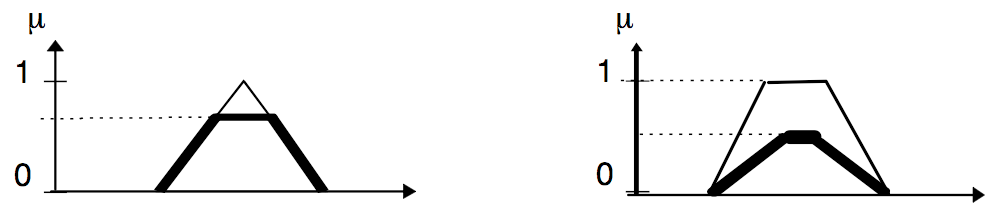
\includegraphics[width=3.45in]{figs/MaxProd.png}
\caption{Activation methods: Min (left) and Prod (right).}
\label{f:activation}
\end{figure}

Finally, aggregation method defines how the consequents from multiple rules are combined within a Rule Block (see Fig.~\ref{f:acumulation}).
Aggregation operators defined in the norm include:  Maximum, Bounded sum, Normed sum, Probabilistic OR, and Sum.

\begin{figure}[!t]
\centering
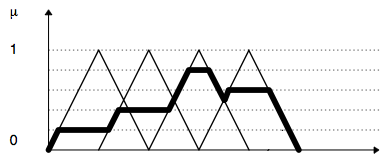
\includegraphics[width=3.45in]{figs/accumulation.png}
\caption{Aggregation method: Combining consequents from multiple rules using ‘Max’ method.}
\label{f:acumulation}
\end{figure}

Only two membership functions are defined in the IEC standard: singleton and piece-wise linear.
jFuzzyLogic also implements other commonly used membership functions: trapezoidal, sigmoidal, gaussian, generalized bell, difference of sigmoidal, and cosine.
Furthermore, jFuzzyLogic allows to build arbitrary membership functions by combining mathematical functions.

Because of the flexibility in defining membership functions, we discretize them at a number of points.
The number of points, by default one thousand, can be adjusted according to the precision-speed trade-off required for a particular application.
Inference is performed by evaluating membership functions at these discretization points.
In order to perform a discretization, the ``universe" for each variable, has to be estimated. 
The universe is defined as the range where the variable has non-neglectable value. 
For each variable, each membership function and each term is taken into account when calculating a universe.
Once all rules have been analyzed, the aggregation for each variable is complete. 

The last step when evaluating a FIS is defuzzification.
The value for each variable is calculated using the selected defuzzification method, which can be 'Center of gravity', 'Rightmost Max', 'Center of area', 'Leftmost Max', 'Mean max' (continuous membership functions), or 'Center of gravity' (discrete membership functions). 

\subsection{API extensions \label{sec:ext}}

Some of the extensions and benefits provided by jFuzzyLogic are described in this section.

\textit{Modularity.} Modular design allows to extend the language and the API easily. It is possible to add custom combination, activation or aggregation methods, defuzzifiers, or membership functions by extending the provided object tree. 

%\begin{figure}[!t]
%\centering
%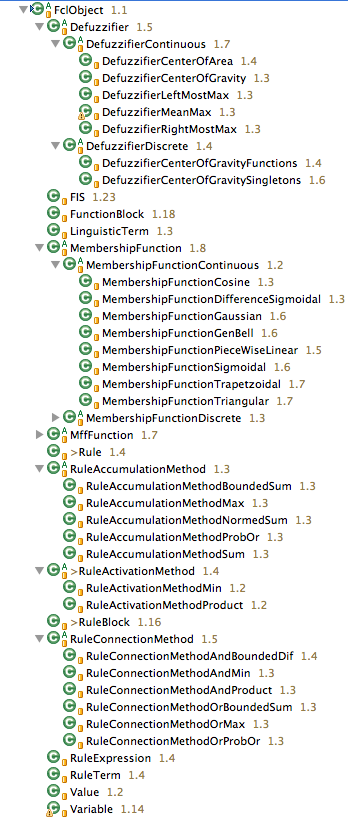
\includegraphics[width=3.45in]{figs/jFuzzy_object_tree.png}
%\caption{jFuzzyLogic object tree provides many extension points.}
%\label{f:tree}
%\end{figure}

\textit{Dynamic changes.} Our API supports dynamic changes made onto a fuzzy inference system: i) variables can be used as membership function parameters; ii) rules can be added or deleted from rule blocks, iii) rule weights can be modified; iv) membership functions can use combinations of pre-defined functions. 

\textit{Optimization API.} An optimization API is available, allowing fine tuning membership function rules and rule weights.
A few optimization algorithms are already implemented, such as gradient descent, partial derivative, and delta algorithm.
Other optimization algorithms can be implemented based on these templates.

%\begin{figure}[!t]
%\centering
%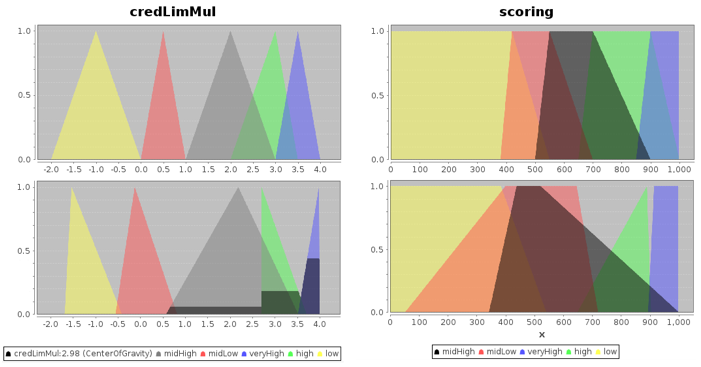
\includegraphics[width=3.5in]{figs/optimization.png}
%\caption{Optimization example: Parameters before (top) and after(bottom) optimization. Top of membership function midHigh overlaps with midLow after variable scoring is optimized, this indicates some potential contradictions between the rule set and the error model.}
%\label{f:optimization}
%\end{figure}

\textit{Data Types.} Due to the nature of fuzzy systems and in order to reduce complexity, jFuzzyLogic considers each variable as \textit{REAL} variable which is mapped to a \textit{double} Java type.

\textit{Excecution order.} By default it is assumed that a FIS is composed of only one Function Block, so evaluating the FIS means evaluating the default FB. 
If a FIS has more than one FB, they are evaluated in alphabetical order by FB name. 
Other execution orders can be implemented by the user, which allows us to define easily hierarchical controllers.

\section{A case study}
\label{sec:cas}

We present an example of creating an FLC controller with jFuzzyLogic.
This case study is focused on the development of the wall following robot as explained in \cite{mucientes2009learning}.
Wall following behavior is well known in mobile robotics. 
It is frequently used for the exploration of unknown indoor environments and for the navigation between two points in a map. 

The main requirement of a good wall-following controller is to maintain a suitable distance from the wall that is being followed. 
The robot should also move as fast as possible, while avoiding sharp movements, making smooth and progressive turns and changes in velocity.

In our fuzzy control system, the input variables are: 
	i) normalized distances from the robot to the right ($RD$) and left walls ($DQ$); 
	ii) orientation with respect to the wall ($O$); and 
	iii) linear velocity ($V$). 
The output variables in this controller are the normalized linear acceleration ($LA$) and the angular velocity ($AV$). 
The linguistic partitions are shown in Fig.~\ref{f:robotVars} which are comprised by linguistic terms with uniformly distributed triangular membership functions giving meaning to them.

\begin{figure}[!t]
\centering
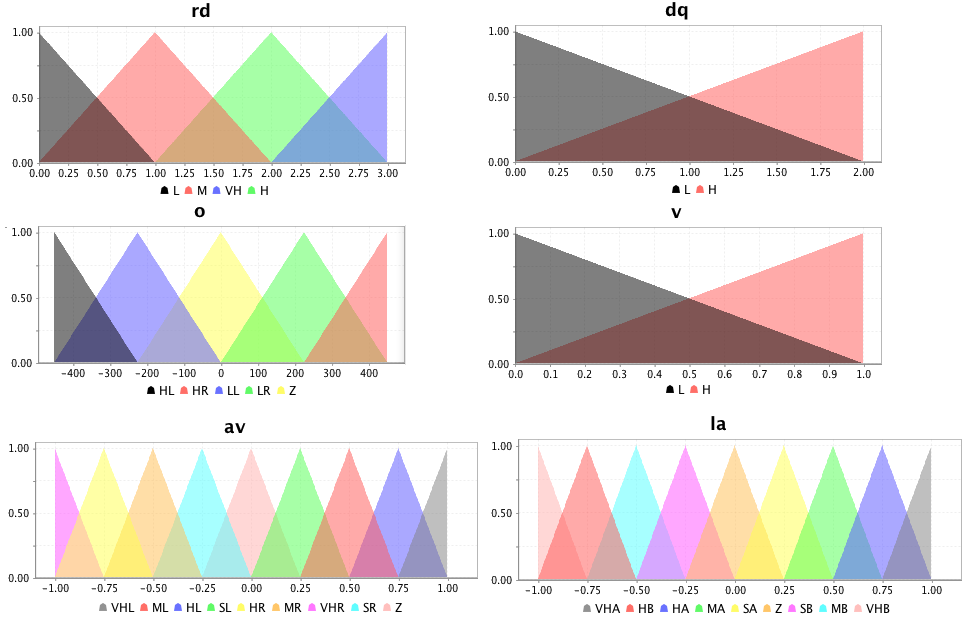
\includegraphics[width=3.5in]{figs/robot_vars_2.png}
\caption{Membership functions for wall-following robot.}
\label{f:robotVars}
\end{figure}

In order to implement the controller, the first step is to declare the input and output variables and to define the fuzzy sets (Table \ref{t:robotVars}).
Variables are defined in \textit{VAR\_INPUT} and \textit{VAR\_OUTPUT} sections.
Fuzzy sets are defined in \textit{FUZZIFY} blocks for input variables and \textit{DEFUZZIFY} blocks for output variables.

One \textit{FUZZIFY} block is used for each input variable.
Each \textit{TERM} line within a \textit{FUZZIFY} block defines a linguistic term and its corresponding membership function. 
In this example all membership functions are triangular, so they are defined using the \textit{'trian'} keyword, followed by three parameters defining left, center and right points (e.g. \textit{`trian 1 2 3'}).

Output variables define their membership functions within \textit{DEFUZZIFY} blocks.
Linguistic terms and membership functions are defined using the \textit{TERM} keyword as previously described for input variables.
In this case we also add parameters to select the defuzzyfication method. 
The statement \textit{'METHOD : COG'} indicates that we are using 'Center of gravity'.

\begin{table*}[!t]
\renewcommand{\arraystretch}{1.3}
\caption{Wall following robot: Fuzzy controller in FCL language: Variable definitions.}
\label{t:robotVars}
\centering
\begin{tabular}{|l|}
\hline
\begin{lstlisting}
VAR_INPUT
	rd : REAL;			// Right distance
	dq : REAL;			// Distance quotient
	o  : REAL;			// Orientation. Note: 'or' is a reserved word
	v  : REAL;			// Velocity
END_VAR

VAR_OUTPUT
	la : REAL;			// Linear acceleration
	av : REAL;			// Angular velocity
END_VAR

FUZZIFY rd
	TERM L  := trian 0 0 1;
	TERM M  := trian 0 1 2;
	TERM H  := trian 1 2 3;
	TERM VH := trian 2 3 3;
END_FUZZIFY

FUZZIFY dq
	TERM L := trian 0 0 2;
	TERM H := trian 0 2 2;
END_FUZZIFY

FUZZIFY o
	TERM HL := trian -450 -450 -225;
	TERM LL := trian -450 -225 0;
	TERM Z  := trian -225 0 225;
	TERM LR := trian 0 225 450;
	TERM HR := trian 225 450 450;
END_FUZZIFY

FUZZIFY v
	TERM L := trian 0 0 1;
	TERM H := trian 0 1 1;
END_FUZZIFY

DEFUZZIFY la
	TERM VHB := trian -1 -1 -0.75;
	TERM HB  := trian -1 -0.75 -0.5;
	TERM MB  := trian -0.75 -0.5 -0.25;
	TERM SB  := trian -0.5 -0.25 0;
	TERM Z   := trian -0.25 0 0.25;
	TERM SA  := trian 0 0.25 0.5;
	TERM MA  := trian 0.25 0.5 0.75;
	TERM HA  := trian 0.5 0.75 1;
	TERM VHA := trian 0.75 1 1;
	METHOD : COG;			// Center of Gravity
	DEFAULT := 0;
END_DEFUZZIFY

DEFUZZIFY av
	TERM VHR := trian -1 -1 -0.75;
	TERM HR  := trian -1 -0.75 -0.5;
	TERM MR  := trian -0.75 -0.5 -0.25;
	TERM SR  := trian -0.5 -0.25 0;
	TERM Z   := trian -0.25 0 0.25;
	TERM SL  := trian 0 0.25 0.5;
	TERM ML  := trian 0.25 0.5 0.75;
	TERM HL  := trian 0.5 0.75 1;
	TERM VHL := trian 0.75 1 1;
	METHOD : COG;
	DEFAULT := 0;
END_DEFUZZIFY

\end{lstlisting} \\
\hline
\end{tabular}
\end{table*}

These membership functions can be plotted by running jFuzzyLogic with an FCL file, having the code shown in Table~ \ref{t:robotVars},  as argument (e.g. \texttt{java -jar jFuzzyLogic.jar robot.fcl}). 
The corresponding FCL file for this case study is available for download as one of the examples provided in jFuzzyLogic package (\texttt{jfuzzylogic.sourceforge.net}).

The second step is to define the rules used for inference. 
They are defined in \textit{RULEBLOCK} statements.
For the wall-following robot controller, we used 'minimum' connection method (\textit{AND : MIN}), minimum activation method (\textit{ACT : MIN}), and maximum aggregation method (\textit{ACCU : MAX}). 
We implemented the rule base generated in~\cite{mucientes2009learning} by the WCOR method~\cite{Alc06}. 
Each entry in the rule base was converted to a single FCL rule (Table~\ref{t:robotRules}).
Within each rule, the antecedent (i.e. the \textit{IF} part) is composed of the input variables connected by \textit{`AND'} operators.
Since there are more than one output variable, we can specify multiple consequents (i.e. \textit{THEN} part) separated by semicolons. 
Finally, we add the desired weight using the \textit{`with'} keyword followed by the weight. 
This completes the implementation of a controller for a wall-following robot using FCL and jFuzzyLogic.

\begin{table*}[!t]
\renewcommand{\arraystretch}{1.3}
\caption{Wall following robot. Fuzzy controller in FCL language: Rule block.}
\label{t:robotRules}
\centering
\begin{tabular}{|l|}
\hline
\begin{lstlisting}
RULEBLOCK rules
	AND  : MIN;			// Use 'min' for 'and' (also implicit use 'max' for 'or' to fulfill DeMorgan's Law)
	ACT  : MIN;			// Use 'min' activation method
	ACCU : MAX;			// Use 'max' aggregation method

    RULE 01:    IF rd is  L and dq is L and o is LL and v is L THEN la is VHB , av is VHR with 0.4610;
    RULE 02:    IF rd is  L and dq is L and o is LL and v is H THEN la is VHB , av is VHR with 0.4896;
    RULE 03:    IF rd is  L and dq is L and o is  Z and v is L THEN la is   Z , av is  MR with 0.6664;
    RULE 04:    IF rd is  L and dq is L and o is  Z and v is H THEN la is  HB , av is  SR with 0.5435;
    RULE 05:    IF rd is  L and dq is H and o is LL and v is L THEN la is  MA , av is  HR with 0.7276;
    RULE 06:    IF rd is  L and dq is H and o is  Z and v is L THEN la is  MA , av is  HL with 0.4845;
    RULE 07:    IF rd is  L and dq is H and o is  Z and v is H THEN la is  HB , av is  ML with 0.5023;
    RULE 08:    IF rd is  L and dq is H and o is LR and v is H THEN la is VHB , av is VHL with 0.7363;
    RULE 09:    IF rd is  L and dq is H and o is HR and v is L THEN la is VHB , av is VHL with 0.9441;
    RULE 10:    IF rd is  M and dq is L and o is  Z and v is H THEN la is  SA , av is  HR with 0.3402;
    RULE 11:    IF rd is  M and dq is L and o is LR and v is H THEN la is   Z , av is VHL with 0.4244;
    RULE 12:    IF rd is  M and dq is L and o is HR and v is L THEN la is  SA , av is  HL with 0.5472;
    RULE 13:    IF rd is  M and dq is L and o is HR and v is H THEN la is  MB , av is VHL with 0.4369;
    RULE 14:    IF rd is  M and dq is H and o is HL and v is L THEN la is   Z , av is VHR with 0.1770;
    RULE 15:    IF rd is  M and dq is H and o is HL and v is H THEN la is VHB , av is VHR with 0.4526;
    RULE 16:    IF rd is  M and dq is H and o is LL and v is H THEN la is  SA , av is VHR with 0.2548;
    RULE 17:    IF rd is  M and dq is H and o is  Z and v is L THEN la is  HA , av is   Z with 0.2084;
    RULE 18:    IF rd is  M and dq is H and o is LR and v is L THEN la is  HA , av is VHL with 0.6242;
    RULE 19:    IF rd is  M and dq is H and o is LR and v is H THEN la is  SA , av is VHL with 0.3779;
    RULE 20:    IF rd is  M and dq is H and o is HR and v is L THEN la is   Z , av is VHL with 0.6931;
    RULE 21:    IF rd is  M and dq is H and o is HR and v is H THEN la is VHB , av is VHL with 0.7580;
    RULE 22:    IF rd is  H and dq is L and o is  Z and v is L THEN la is  HA , av is VHR with 0.5758;
    RULE 23:    IF rd is  H and dq is L and o is LR and v is H THEN la is  SA , av is  MR with 0.2513;
    RULE 24:    IF rd is  H and dq is L and o is HR and v is L THEN la is  HA , av is VHL with 0.5471;
    RULE 25:    IF rd is  H and dq is L and o is HR and v is H THEN la is  SA , av is  HL with 0.5595;
    RULE 26:    IF rd is  H and dq is H and o is HL and v is L THEN la is VHB , av is VHR with 0.9999;
    RULE 27:    IF rd is  H and dq is H and o is HL and v is H THEN la is VHB , av is VHR with 0.9563;
    RULE 28:    IF rd is  H and dq is H and o is LL and v is L THEN la is  HA , av is VHR with 0.9506;
    RULE 29:    IF rd is  H and dq is H and o is  Z and v is L THEN la is  HA , av is VHR with 0.4529;
    RULE 30:    IF rd is  H and dq is H and o is  Z and v is H THEN la is  SA , av is VHR with 0.2210;
    RULE 31:    IF rd is  H and dq is H and o is LR and v is L THEN la is  HA , av is  MR with 0.3612;
    RULE 32:    IF rd is  H and dq is H and o is LR and v is H THEN la is  SA , av is  MR with 0.2122;
    RULE 33:    IF rd is  H and dq is H and o is HR and v is L THEN la is  HA , av is  HL with 0.7878;
    RULE 34:    IF rd is  H and dq is H and o is HR and v is H THEN la is  SA , av is VHL with 0.3859;
    RULE 35:    IF rd is VH and dq is L and o is LR and v is L THEN la is  HA , av is VHR with 0.5530;
    RULE 36:    IF rd is VH and dq is L and o is HR and v is L THEN la is  HA , av is  HR with 0.4223;
    RULE 37:    IF rd is VH and dq is L and o is HR and v is H THEN la is  SA , av is  HR with 0.3854;
    RULE 38:    IF rd is VH and dq is H and o is LL and v is L THEN la is  HA , av is VHR with 0.0936;
    RULE 39:    IF rd is VH and dq is H and o is LR and v is L THEN la is  HA , av is VHR with 0.7325;
    RULE 40:    IF rd is VH and dq is H and o is LR and v is H THEN la is  SA , av is VHR with 0.5631;
    RULE 41:    IF rd is VH and dq is H and o is HR and v is L THEN la is  HA , av is  HR with 0.5146;
END_RULEBLOCK
\end{lstlisting} \\
\hline
\end{tabular}
\end{table*}

\section{Conclusions}
\label{sec:con}

In this paper, we have described jFuzzyLogic, an open source Java library for fuzzy systems which allow us to design FLCs following the standard IEC 61131.
It allows us to reduce programming work and extend the range of possible users applying fuzzy systems and FLCs.

We have shown a case study to illustrate the use of jFuzzyLogic. 
In this case, we developed an FLC controller for wall-following behavior in a robot.
The example shows how FCL can be used to easily implement fuzzy logic systems.

The jFuzzyLogic software package is continuously being updated and improved. 
At the moment, we are developing an implementation of a C/C++ compiler for fuzzy inference systems. 
This will allow easy implementation with embedded control systems using different processors.

% \subsection{Subsection Heading Here}
% Subsection text here.


% \subsubsection{Subsubsection Heading Here}
% Subsubsection text here.


% An example of a floating figure using the graphicx package.
% Note that \label must occur AFTER (or within) \caption.
% For figures, \caption should occur after the \includegraphics.
% Note that IEEEtran v1.7 and later has special internal code that
% is designed to preserve the operation of \label within \caption
% even when the captionsoff option is in effect. However, because
% of issues like this, it may be the safest practice to put all your
% \label just after \caption rather than within \caption{}.
%
% Reminder: the "draftcls" or "draftclsnofoot", not "draft", class
% option should be used if it is desired that the figures are to be
% displayed while in draft mode.
%
%\begin{figure}[!t]
%\centering
%\includegraphics[width=3.45in]{myfigure}
% where an .eps filename suffix will be assumed under latex, 
% and a .pdf suffix will be assumed for pdflatex; or what has been declared
% via \DeclareGraphicsExtensions.
%\caption{Simulation Results}
%\label{fig_sim}
%\end{figure}

% Note that IEEE typically puts floats only at the top, even when this
% results in a large percentage of a column being occupied by floats.


% An example of a double column floating figure using two subfigures.
% (The subfig.sty package must be loaded for this to work.)
% The subfigure \label commands are set within each subfloat command, the
% \label for the overall figure must come after \caption.
% \hfil must be used as a separator to get equal spacing.
% The subfigure.sty package works much the same way, except \subfigure is
% used instead of \subfloat.
%
%\begin{figure*}[!t]
%\centerline{\subfloat[Case I]\includegraphics[width=3.45in]{subfigcase1}%
%\label{fig_first_case}}
%\hfil
%\subfloat[Case II]{\includegraphics[width=3.45in]{subfigcase2}%
%\label{fig_second_case}}}
%\caption{Simulation results}
%\label{fig_sim}
%\end{figure*}
%
% Note that often IEEE papers with subfigures do not employ subfigure
% captions (using the optional argument to \subfloat), but instead will
% reference/describe all of them (a), (b), etc., within the main caption.


% An example of a floating table. Note that, for IEEE style tables, the 
% \caption command should come BEFORE the table. Table text will default to
% \footnotesize as IEEE normally uses this smaller font for tables.
% The \label must come after \caption as always.
%
%\begin{table}[!t]
%% increase table row spacing, adjust to taste
%\renewcommand{\arraystretch}{1.3}
% if using array.sty, it might be a good idea to tweak the value of
% \extrarowheight as needed to properly center the text within the cells
%\caption{An Example of a Table}
%\label{table_example}
%\centering
%% Some packages, such as MDW tools, offer better commands for making tables
%% than the plain LaTeX2e tabular which is used here.
%\begin{tabular}{|c||c|}
%\hline
%One & Two\\
%\hline
%Three & Four\\
%\hline
%\end{tabular}
%\end{table}


% Note that IEEE does not put floats in the very first column - or typically
% anywhere on the first page for that matter. Also, in-text middle ("here")
% positioning is not used. Most IEEE journals/conferences use top floats
% exclusively. Note that, LaTeX2e, unlike IEEE journals/conferences, places
% footnotes above bottom floats. This can be corrected via the \fnbelowfloat
% command of the stfloats package.

% conference papers do not normally have an appendix

% use section* for acknowledgement
\section*{Acknowledgment}

jFuzzyLogic was designed and developed by P. Cingolani. 
He is supported in part by McGill Uninversity, Genome Quebec.
J. Alcala-Fdez is supported by the Spanish Ministry of Education and Science under Grant TIN2011-28488 and the Andalusian Government under Grant P10-TIC-6858. 

We would like to thank R. Sladek and M. Blanchette for their comments. Special thanks to P.J. Leonard for his contributions to the project.

% trigger a \newpage just before the given reference
% number - used to balance the columns on the last page
% adjust value as needed - may need to be readjusted if
% the document is modified later
%\IEEEtriggeratref{8}
% The "triggered" command can be changed if desired:
%\IEEEtriggercmd{\enlargethispage{-5in}}

%---
% References section
%---
\bibliographystyle{IEEEtran}
% argument is your BibTeX string definitions and bibliography database(s)
\bibliography{IEEEabrv,CingolaniAlcala-Fdez-FuzzIEEE2012}

% that's all folks
\end{document}


